\section{Methodology}


In this section, using trade flow data for the year 2022, along with specifications from the IHS dataset, we will perform data analysis.

Tradetable data is available in the trade flow dataset. For each segments there is trade flow and therefore we will have to perform the analysis for each segment separately.

The steps involved in the analysis are as follows:

\begin{figure}[h]
    \centering
    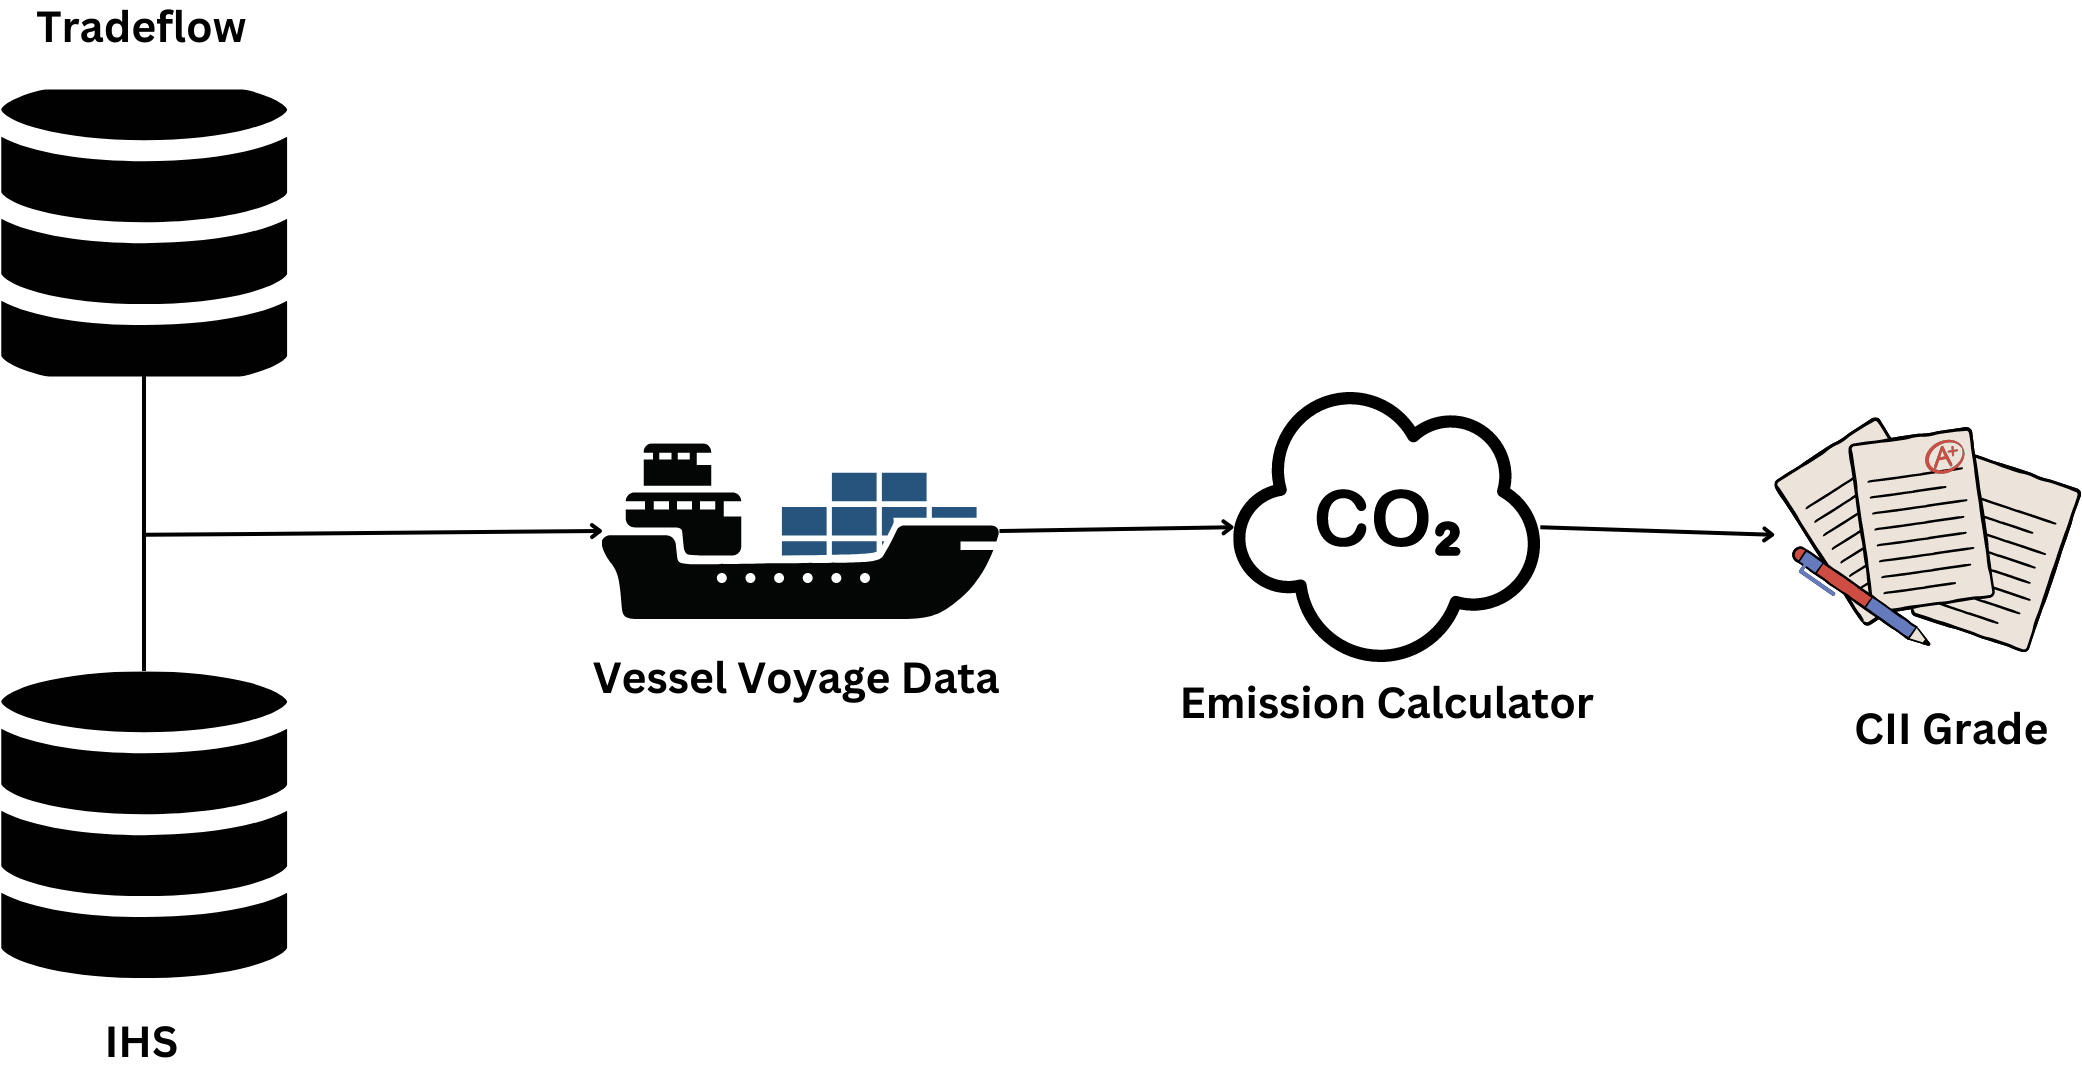
\includegraphics[width=0.5\textwidth]{images/methodlogy.png}
    \caption{Methodology Overview}
    \label{methodlogy}
\end{figure}

\newpage

\subsubsection{1. Getting distinct IMO numbers from trade flow}

Distinct IMO (International Maritime Organization) numbers were obtained from the trade flow dataset by querying the texttt{imo} column. 
This process helped in identifying all the unique ships present in the dataset, forming the foundation for further analysis.


\subsubsection{2. Getting necessary information for each IMO number from IHS and trade flow}

For each distinct IMO number identified in the previous step, the IHS dataset was queried or joined with trade flow to gather relevant information about each ship. 
This included details such as specifications, fuel type, engine types, and more. 
The process consisted of the following steps:

\begin{itemize}
    \item \textbf{Estimating Cargo Based on Draught:} Cargo was estimated using the draught noted on ports and the maximum draught from the IHS dataset. This allowed for an understanding of the cargo load for different vessels.
    
    \item \textbf{Determining Laden or Ballast Trade Flows:} The trade flows were categorized into laden or ballast based on the ballast threshold percentage from segment parameters. This categorization assisted in differentiating the vessel's operational conditions.
    
    \item \textbf{Converting to Pandas DataFrame:} The obtained shipTrade data was converted into a Pandas DataFrame, facilitating further processing and analysis.
    
    \item \textbf{Dividing into DataFrames for Laden and Ballast Trade Flows:} The trade data was divided into separate DataFrames for laden and ballast trade flows. This segmentation enabled focused analysis on different operational conditions.
    
    \item \textbf{Extracting Information on Distance, Time, and Average Speed:} Information such as distance, time, and average speed was extracted for both ballast and laden trade flows. These parameters provided insights into the efficiency and operation of the vessels.
    
    \item \textbf{Calculating Cargo:} The total cargo was calculated based on laden trade data, contributing to the overall understanding of the vessels' capacity and utilization.
\end{itemize}



\subsubsection{3. Cleaning data}

Data cleaning is a critical step in the methodology, ensuring that the dataset is ready for analysis. This involves handling missing values, removing duplicates, standardizing units, and correcting any inconsistencies. Specific aspects of the data cleaning process included:


\begin{itemize}
    \item \textbf{Handling Missing Speed Values:} In some cases, the average speed determined from AIS (Automatic Identification System) data might be missing or unusually high for specific trade flows. To address this, the distance and time values were used to calculate the average speed, ensuring that the analysis was based on consistent and realistic speed data.
    
    \item \textbf{Excluding Trades with Missing Distance:} Any trades with missing average distance values were excluded from the analysis. This helped maintain the integrity and accuracy of the dataset.
    
\end{itemize}


Sometimes for certain trades average distance was missing, this trades were excluded.

\subsubsection{4. Calculating emissions for laden and ballast tradeflows.}

The calculation of emissions for laden and ballast trade flows was a central component of the methodology. Utilizing the information extracted in the previous steps, the emissions were calculated using the AFC (Automated Flight Control) emission calculator API. Here's how the process was executed:

\begin{itemize}
    \item \textbf{Emission Calculation Function:} A specific function, getEmission, was employed to calculate emissions. This function took essential parameters like IMO number, cargo amount, distance, load condition, and estimated speed as input.
    
    \item \textbf{API Request:} The function made a request to the AFC emission calculator API, passing the required parameters. The response from the API included detailed emission data, providing insights into various emission aspects such as CO2, SO2, NO2, and others.
    \item 
    \item \textbf{Error Handling:} The process included robust error handling to manage any issues with the API request, ensuring that the analysis was not disrupted by unexpected errors or inconsistencies.
    
    
\end{itemize}

\subsubsection{5. Calculating CII, CII required, and CII reference.}

Carbon Intensity Indicator (CII) is calculated as the ratio of emissions (CO\textsubscript{2}) to transport work (distance traveled $\times$ cargo amount). CII required is based on regulatory standards, while CII reference can be derived from historical data or benchmarks. Calculate these indicators for each trade flow using the emission data and transport work values.

CII reference is calculated using the following formula:

\begin{equation}
    CII_{\text{ref}} = a \cdot \text{Capacity}^{-C}
\end{equation}

where $a$ and $C$ are constants according to Figure \ref{cii_ref_constant}, and Capacity is the deadweight of the ship.

\begin{figure}[h]
    \centering
    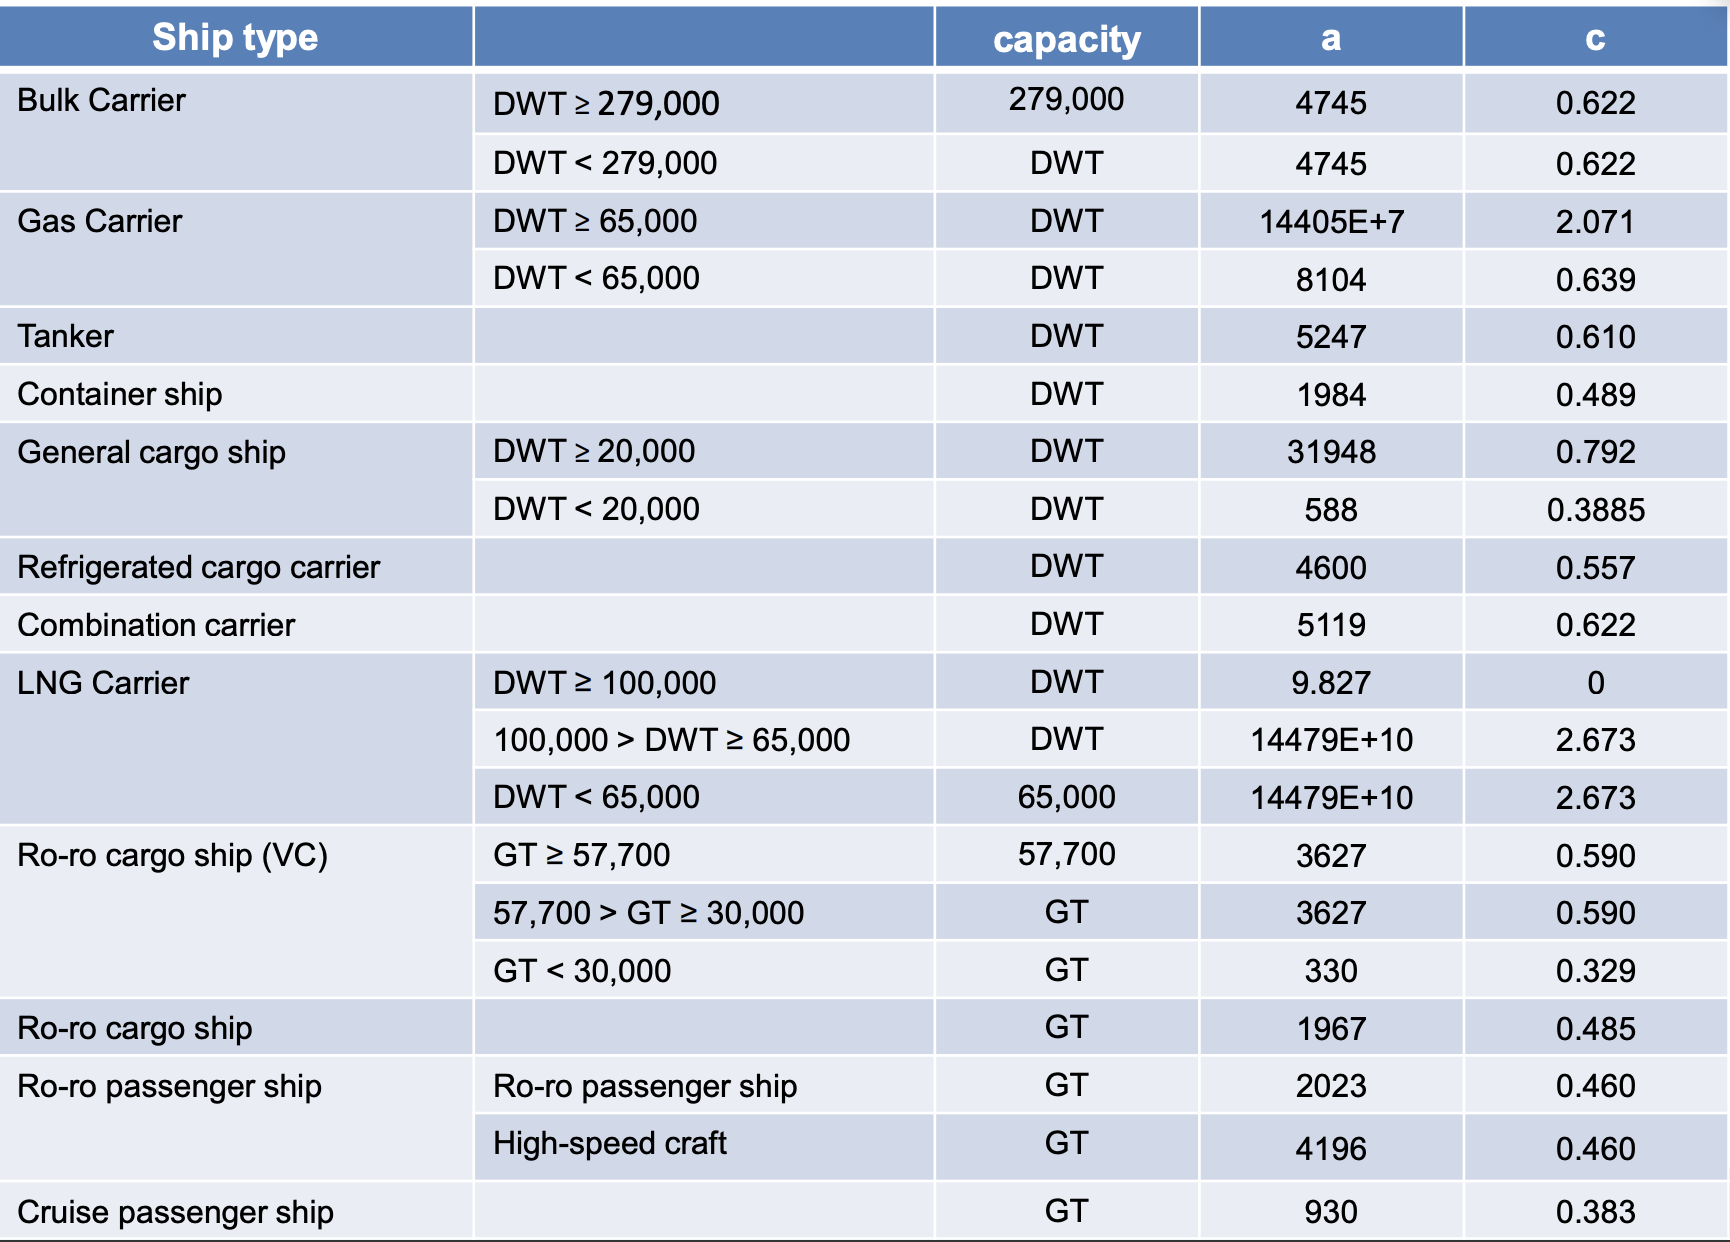
\includegraphics[width=1\textwidth]{images/cii_ref_constant.png}
    \caption{$a$ and $C$ constants}
    \label{cii_ref_constant}
\end{figure}

CII required can be calculated using the following formula:

\begin{equation}
    \text{Requited CII} = \left( \frac{100 -Z}{100}\right) \times \text{CIIRef}
    \label{cii_required}
\end{equation}

In Equation 5.2, the reduction factor Z represents the initial value of 5\% in the year 2023,
with an annual increment of 2\%. Additionally, for the years 2027 to 2030,
the Z factors are subject to enhancement and refinement, guided by the evaluation of the short-term measure's effectiveness.

\newpage

\begin{table}[htbp]
    \centering
    \begin{tabular}{cc}
        \toprule
        Year & Reduction Factor (Z) \\
        \midrule
        2023 & 5\%                  \\
        2024 & 7\%                  \\
        2025 & 9\%                  \\
        2026 & 11\%                 \\
        2027 & **                   \\
        2028 & **                   \\
        2029 & **                   \\
        2030 & **                   \\
        \bottomrule
    \end{tabular}
    \caption{Reduction Factors Over the Years}
    \label{tab:reduction-factors}
\end{table}

\subsubsection{6. Calculating CII grade.}

Based on the calculated CII and CII required, determine the CII grade for each trade flow, indicating its compliance with emissions regulations.
This can be done using predefined thresholds or standards to categorize trade flows into different CII grades.

Taking into account that vessels will experience similar voyages in 2023 as they did in 2022, the CII grade for the end of 2023 can be estimated with a reduction factor Z set at 5.

The $"dd"$ vector is established by calculating the ratio between Attained CII and Required CII.
This ratio is subsequently compared against the thresholds for CII grades to ascertain the appropriate grade.
The larger the deviation of the ratio, the lower the grade assigned, with A representing the best and E signifying the poorest performance.


\begin{figure}[h]
    \centering
    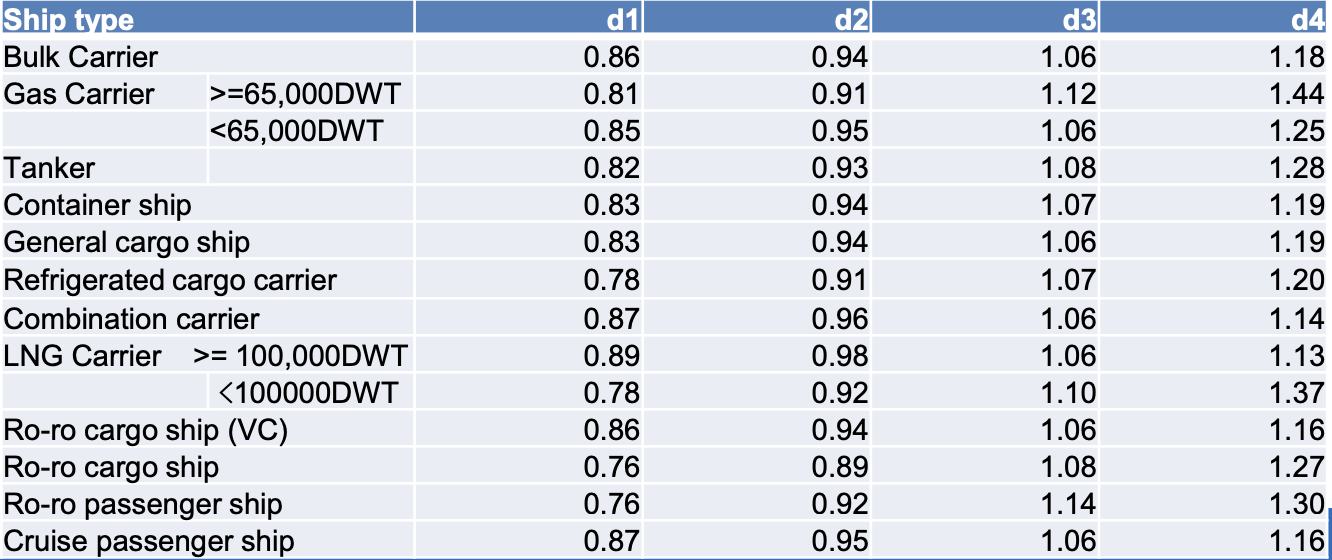
\includegraphics[width=1\textwidth]{images/dd_vecotor.png}
    \caption{$dd$ vectors for determining the rating boundaries of ship types}
    \label{dd_vecotor}
\end{figure}

\begin{figure}[h]
    \centering
    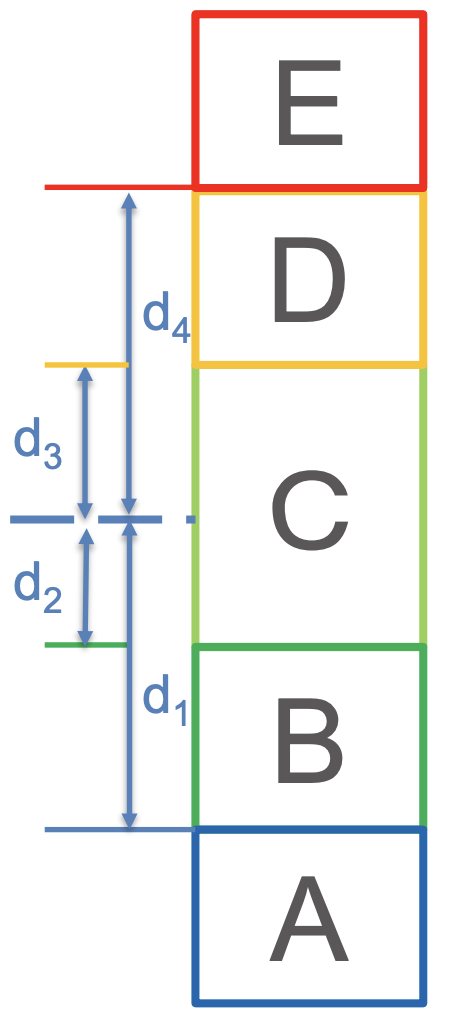
\includegraphics[width=0.2\textwidth]{images/cii_grade_dd_grade.png}
    \caption{CII grading based on $dd$ vector}
    \label{cii_grade_dd_grade}
\end{figure}

Based on figure \ref{dd_vecotor}, the CII grade can be determined as represented in figure \ref{cii_grade_dd_grade}.


Following above 6 steps, we can calculate emissions, CII, CII required, CII reference and CII grade for each vessel.
Results can be stored in a SQL table for further analysis.
For each segment, we can perform above steps as showing in Listing \ref{analysis_segment}

\begin{lstlisting}[language=python, caption=Analysis for capsize segment, label=analysis_segment]
    capsizeImoQeury = spark.sql(f"""
                       select distinct(imo) from capesize.tradeFlow as st
                       """)
    startDate = '2022-01-01'
    endDate = '2022-12-31'
    segment = 'capesize'
    capeSize = capsizeImoQeury.toPandas()
    for imo in capeSize['imo']:
    imoCIIData = getCIIGradeByImo(imo, startDate, endDate, segment, 5)
    df = pd.DataFrame([imoCIIData])
    spark.createDataFrame(df).write.mode("append").saveAsTable("emissions.capesize_cii_2022_v3")
    time.sleep(5)
\end{lstlisting}

In listing \ref{analysis_segment}, we are getting distinct IMO numbers for capsize segment.
Then for each IMO number, we are calling \texttt{getCIIGradeByImo} function to get emissions, CII, CII required, CII reference and CII grade.
Using $spark.createDataFrame(df).write()$ we are storing results in SQL table.

Based on the data obtained so far, we will analysis the results in the next chapter.